\noindent
% We propose to extend Nek5000/RS and NekROM to support a multiscale simulation
% environment.   The first set of tasks will be to provide more seemless
% integration between Nek5000/RS and NekROM.  Ideally, one should be able to
% generate a ROM on the fly.

\vspace{-.1in}
{\bf Proposed Tasks.}
We propose the following tasks to realize a multiscale simulation
capability within Nek5000/RS/ROM for reactor analysis:

\textbf{Thrust 1: Data Generation.} We perform high fidelity simulations of the
flow in SFR fuel assemblies for a variety of conditions including a range of
steady-state conditions and a loss-of-flow transient scenario.
\\[-4ex]
\begin{description}
\item{$\; i.\; \;$}
Define benchmarks for SFR fuel assemblies. These will be used for validation.
\\[-4ex]
\item{$\, ii. \,\;$}
Develop data to construct reduced order models of SFR fuel assemblies. This
task will support Thrust 2.  
\\[-4ex]
\item{\em iii.} Develop data to validate reduced order models for both
transient and parameter sweeps. This Task will support Thrust 3.
\\[-4ex]
\end{description}

\textbf{Thrust 2: Algorithmic Development.} This is the core of the project.
We seek to develop advanced ROM methods that are seemlessly
extended to a multi-scale framework in Nek5000/RS/ROM.
\\[-5ex]
\begin{description}
\item{$\; i.\, \;$}
Continued development of ROM closure models to increase robustness 
for high Rayleigh/Reynolds flows.  This effort will build on the work of
\cite{kaneko22a,kaneko22,tsai22a,kaneko20a}.
\\[-3ex]
\item{$\, ii. \,\;$}
Identify strategies to equip the ROM for long-time transients.  
Proposed extensions to the methods demonstrated in \cite{kaneko20a}
include error-indicated pMOR and improved stabilizing bases.
\\[-3ex]
\item{\em iii.}
Develop multi-scale methods that couple ROMs with LES on a subset of the
domain.  Principal challenges are to support general or parameterized inflow
conditions for the ROM and to quantify relaxation distances over which small
scale structures will evolve near the ROM-LES interface. The goal will be to
combine reactor-scale ROM simulations with localized detailed simulations in
regions of interest. This leverages past work on rod bundles and sub-channels,
whose geometric properties have been exploited to maximize the use of small
domain high-fidelity simulation to improve RANS results in a multi-scale
fashion \cite{martinez2019a}.  
\\[-5ex]
\end{description}%

\textbf{Thrust 3: Validation and Demonstration.} 
Here we validate and demonstrate the proposed methods.
\\[-5ex]
\begin{description}
\item{$\; i.\; \;$}
Validate ROM transient calculations with high-fidelity counterparts
in an SFR rod-bundle under low-flow conditions.
\\[-4ex]
\item{$\, ii. \,\;$}
Perform ROM-based parameter sweeps and compare these to corresponding
FOM results for validation.
\\[-4ex]
\item{\em iii.}
Demonstrate accelerated transient capability for cases that are currently not
feasible. We will implemented the proposed ROM-based and multiscale models within Cardinal \cite{cardinal}. This will enable their usage within the systems analysis code SAM \cite{hu2021}. The co-PI at Penn State has been working extensively on the integration of SAM and NekRS within Cardinal.
\\[-3ex]
\end{description}

\textbf{Major deliverables and Timetable of Activities} \\
At the end of each year a report will be issued describing progress to date.
Four major deliverables are expected out of this project as shown on
Fig.~\ref{fig:gantt}: \\

\vspace*{-.10in}
\noindent \textbf{Thrust 1: Development of Transient High-resolution
Benchmarks} (September 2024). We define at least three transient and parametric
sweep benchmarks for Sodium Fast Reactors. We also provide initial simulation
with LES/DNS using the NEAMS code NekRS. This will be used to support Thrust 3.

\noindent \textbf{Thrust 2: Preliminary Implementation of ROM-based Multiscale
algorithms} (September 2025). Preliminary implementations are discussed. A
comparison against initial benchmark problems is provided. Issues with the
methods are highlighted as well as possible solutions.

\noindent \textbf{Thrust 2/3: Final Implementation and Demonstration of
ROM-based Multiscale Algorithms} (September 2026). 
Culmination of the project. Improvement implementations are discussed. We
provide recommendations on how the methods are to be integrated within the
NEAMS program.

\noindent \textbf{Code Release.} (September 2026). The production code is
released in public repositories.

%\begin{table}[tbhp]
%\begin{center}
%\caption{Timeline of proposal (in months)}
%\centering
%\label{tab:wbs}
%\begin{tabular}{|c|c|c|c|c|c|c|c|c|c|c|}
%\hline
%\textbf{Months} & 1--6&  7--12 & 13--18 & 19--24 & 25--30 & 31--36 & 37--42 & 43--48 & 49--54 & 55--60  \\
%\hline
%\textbf{Task A} & x & x & x & x  & x  & x &   &   &   &  \\
%\hline
%\textbf{Task B} & x & x & x & x  & x  & x &  &   &   &  \\
%\hline
%\textbf{Task C} & x  & x & x & x  & x  & x &   &   &   &  \\
%\hline
%\textbf{Task D} & x  & x  & x  & x  & x  & x & x & x & x & x \\
%\hline
%\textbf{Task E} &   &   &   &   &  x  & x & x & x & x & x \\
%\hline
%\textbf{Task F} &   &   &   &    &  x  & x & x & x & x  & x  \\
%\hline
%\end{tabular}
%\end{center}
%\end{table}

\begin{figure}[t!] \centering
    {\setlength{\unitlength}{1.0in} \begin{picture}(6.5,2.500)(0.0,0)
      \put(0.9,-.10){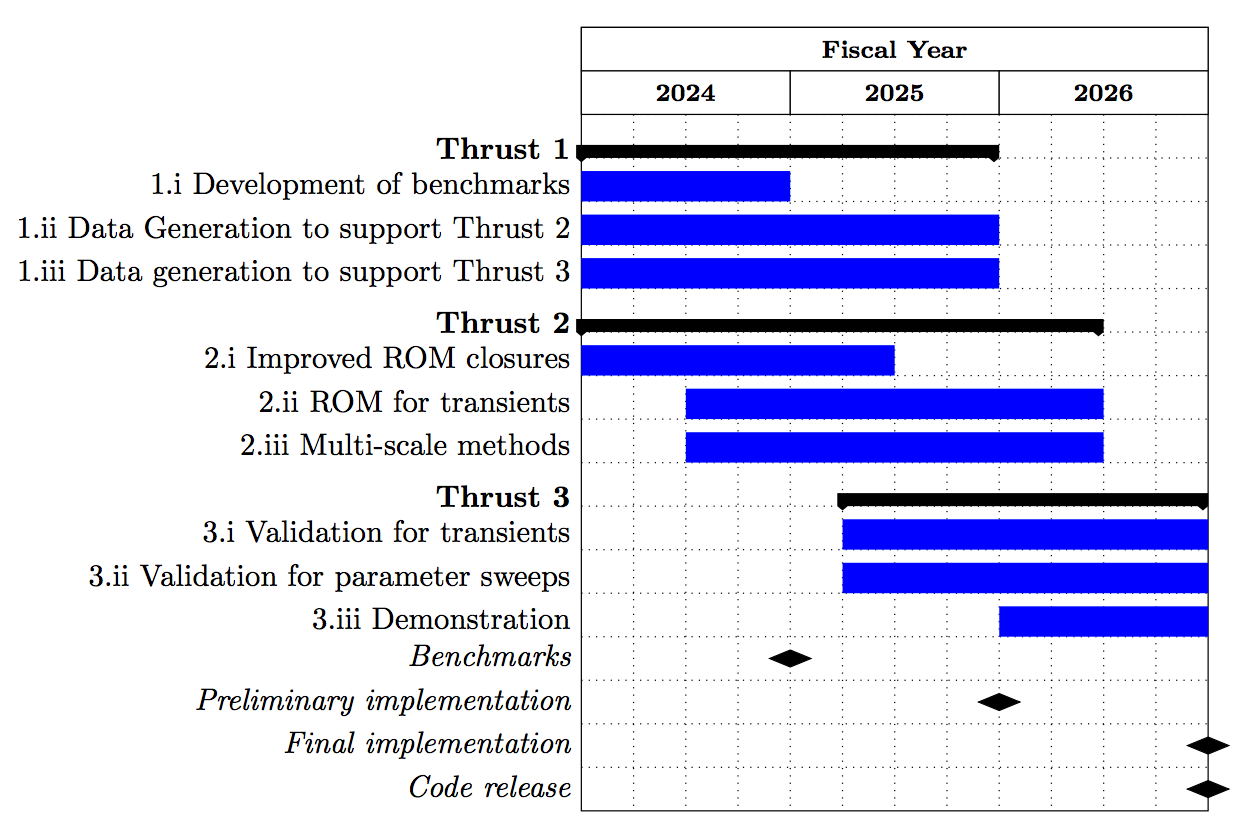
\includegraphics[height=2.7in]{figs/neup_gantt.png}}
    \end{picture}} 
    \caption{Timeline of proposal by fiscal year.  \label{fig:gantt}
\\[-3ex]
}
\end{figure}

%%% \begin{figure} [hbt]
%%% \centering
%%% \begin{ganttchart}[%Specs
%%%  x unit=0.6cm,
%%%  y unit title=0.5cm,
%%%  y unit chart=0.5cm,
%%%  vgrid,hgrid,
%%%  title height=1,
%%% %     title/.style={fill=none},
%%%  title label font=\bfseries\footnotesize,
%%%  bar/.style={fill=blue},
%%%  bar height=0.7,
%%% %   progress label text={},
%%%  group right shift=0,
%%%  group top shift=0.7,
%%%  group height=.3,
%%%  group peaks width={0.2},
%%%  inline]{1}{12}
%%% %labels
%%% \gantttitle[]{Fiscal Year}{12}    \\             % title 2
%%% \gantttitle{2024}{4}
%%% \gantttitle{2025}{4}
%%% \gantttitle{2026}{4}\\
%%% % Setting group if any
%%% \ganttgroup[inline=false]{Thrust 1}{1}{8} \\
%%% \ganttbar[inline=false]{1.i Development of benchmarks}{1}{4} \\
%%% \ganttbar[inline=false]{1.ii Data Generation to support Thrust 2 }{1}{8} \\
%%% \ganttbar[inline=false]{1.iii Data generation to support Thrust 3 }{1}{8} \\
%%% \ganttgroup[inline=false]{Thrust 2}{1}{10} \\
%%% \ganttbar[inline=false]{2.i Improved ROM closures }{1}{6} \\
%%% \ganttbar[inline=false]{2.ii ROM for transients}{3}{10}\\
%%% \ganttbar[inline=false]{2.iii Multi-scale methods}{3}{10} \\
%%% \ganttgroup[inline=false]{Thrust 3}{6}{12} \\
%%% \ganttbar[inline=false]{3.i Validation for transients }{6}{12} \\
%%% \ganttbar[inline=false]{3.ii Validation for parameter sweeps}{6}{12}\\
%%% \ganttbar[inline=false]{3.iii Demonstration}{9}{12} \\
%%% \ganttmilestone[inline=false]{Benchmarks}{4} \\
%%% \ganttmilestone[inline=false]{Preliminary implementation}{8} \\
%%% \ganttmilestone[inline=false]{Final implementation}{12} \\
%%% \ganttmilestone[inline=false]{Code release}{12}
%%% \end{ganttchart}
%%% \caption{Timeline of proposal by fiscal year} \label{fig:gantt}
%%% \end{figure}
%%% %-----------------------------------------------------------------------------
